\documentclass[letterpaper, headinclude, footinclude = true]{article}
\PassOptionsToPackage{noopticals, mathlf}{MinionPro}
\usepackage[minionprospacing, nochapters, beramono, listings, minionpro]{classicthesis}
\usepackage{amsmath}
\usepackage[T1]{fontenc}
\usepackage{microtype}
\usepackage{booktabs}
\usepackage{graphicx}
\usepackage{float}
\usepackage{tikz}



\usepackage{listings}

\lstset{language=[LaTeX]Tex,%C++,
    keywordstyle=\color{RoyalBlue},%\bfseries,
    basicstyle=\small\ttfamily,
    %identifierstyle=\color{NavyBlue},
    commentstyle=\color{Green}\ttfamily,
    stringstyle=\rmfamily,
    numbers=none,%left,%
    numberstyle=\scriptsize,%\tiny
    stepnumber=5,
    numbersep=8pt,
    showstringspaces=false,
    breaklines=true,
    frameround=ftff,
    %frame=single,
    belowcaptionskip=.75\baselineskip
    %frame=L
} 

\usetikzlibrary{shapes,arrows,backgrounds,positioning}

 

\begin{document}
	\section{Simple straight lines} % (fold)
	\label{sec:simple_straight_lines}

\begin{tabular}{p{3cm}l}
\begin{tikzpicture}[baseline = (current bounding box.east)]
	\draw (0,0) -- (1,2);
\end{tikzpicture}
&
\begin{lstlisting}
\begin{tikzpicture}
	\draw (0,0) -- (1,2);
\end{tikzpicture}
\end{lstlisting}	
\\
&
\\
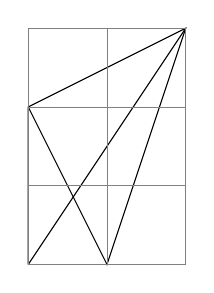
\begin{tikzpicture}[baseline = (current bounding box.east)]
	\draw (0,0) -- (0,2) -- (2,3) -- (1,0) -- (0, 2);
	\draw (0,0) -- (2,3);
	\draw[help lines] (0, 0) grid (2, 3);
\end{tikzpicture}
&
\begin{lstlisting}
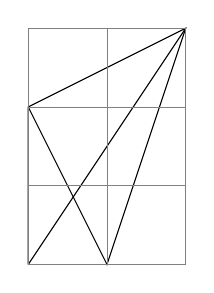
\begin{tikzpicture}
	\draw (0,0) -- (0,2) -- (2,3) -- (1,0) -- (0, 2);
	\draw (0,0) -- (2,3);
	\draw[help lines] (0, 0) grid (2, 3);
\end{tikzpicture}
\end{lstlisting}
\end{tabular}	


\section{Scaling pictures} 
\label{sec:scaling_pictures}
\begin{tabular}{p{3cm}l}
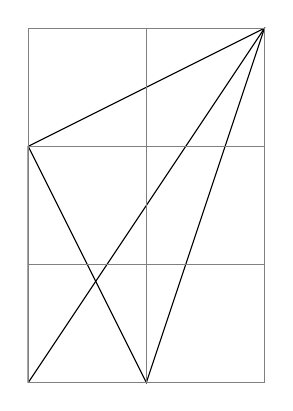
\begin{tikzpicture}[scale = 1.5, baseline = (current bounding box.east)]
	\draw (0,0) -- (0,2) -- (2,3) -- (1,0) -- (0, 2);
	\draw (0,0) -- (2,3);
	\draw[help lines] (0, 0) grid (2, 3);
\end{tikzpicture}
&
\begin{lstlisting}
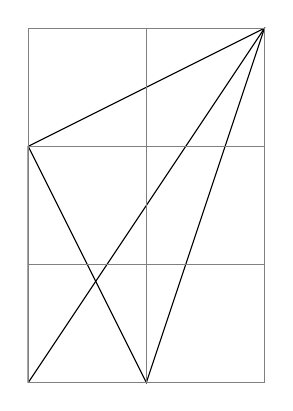
\begin{tikzpicture}[scale = 1.5]
	\draw (0,0) -- (0,2) -- (2,3) -- (1,0) -- (0, 2);
	\draw (0,0) -- (2,3);
	\draw[help lines] (0, 0) grid (2, 3);
\end{tikzpicture}
\end{lstlisting}
\\
&
\\
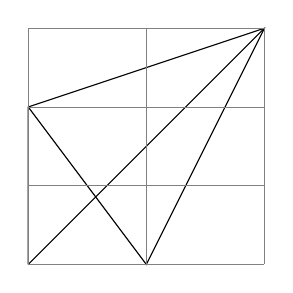
\begin{tikzpicture}[xscale = 1.5, baseline = (current bounding box.east)]
	\draw (0,0) -- (0,2) -- (2,3) -- (1,0) -- (0, 2);
	\draw (0,0) -- (2,3);
	\draw[help lines] (0, 0) grid (2, 3);
\end{tikzpicture}
&
\begin{lstlisting}
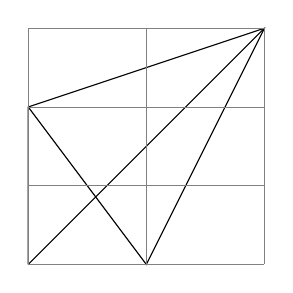
\begin{tikzpicture}[xscale = 1.5]
	\draw (0,0) -- (0,2) -- (2,3) -- (1,0) -- (0, 2);
	\draw (0,0) -- (2,3);
	\draw[help lines] (0, 0) grid (2, 3);
\end{tikzpicture}
\end{lstlisting}
\\
&
\\
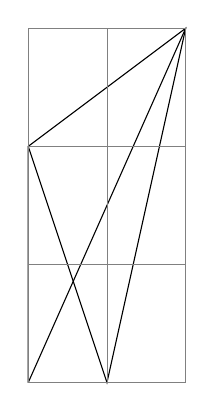
\begin{tikzpicture}[yscale = 1.5, baseline = (current bounding box.east)]
	\draw (0,0) -- (0,2) -- (2,3) -- (1,0) -- (0, 2);
	\draw (0,0) -- (2,3);
	\draw[help lines] (0, 0) grid (2, 3);
\end{tikzpicture}
&
\begin{lstlisting}
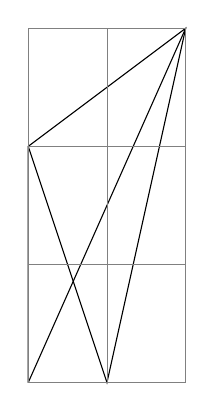
\begin{tikzpicture}[yscale = 1.5]
	\draw (0,0) -- (0,2) -- (2,3) -- (1,0) -- (0, 2);
	\draw (0,0) -- (2,3);
	\draw[help lines] (0, 0) grid (2, 3);
\end{tikzpicture}
\end{lstlisting}
\end{tabular}

\section{Arrows} % (fold)
\label{sec:arrows}
\begin{tabular}{p{3cm}l}

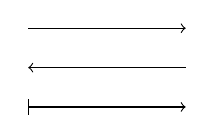
\begin{tikzpicture}[baseline = (current bounding box.east)]
\draw [->] (0,0) -- (2, 0);
\draw [<-] (0, -0.5) -- (2,-0.5);
\draw [|->] (0,-1) -- (2,-1);
\end{tikzpicture}
&
\begin{lstlisting}
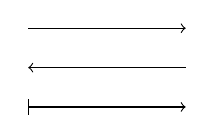
\begin{tikzpicture}
\draw [->] (0,0) -- (2, 0);
\draw [<-] (0, -0.5) -- (2,-0.5);
\draw [|->] (0,-1) -- (2,-1);
\end{tikzpicture}
\end{lstlisting}
\\
&
\\
\begin{tikzpicture}[baseline = (current bounding box.east)]
\draw [<->] (2, 0) -- (0,0) -- (0,2);
\end{tikzpicture}
&
\begin{lstlisting}
\begin{tikzpicture}
\draw [<->] (2, 0) -- (0,0) -- (0,2);
\end{tikzpicture}
\end{lstlisting}
\end{tabular}

\section{Changing thickness} % (fold)
\label{sec:changing_thickness}
\begin{tabular}{p{3cm}l}
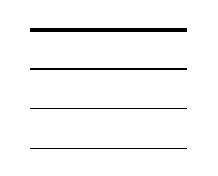
\begin{tikzpicture}[baseline = (current bounding box.east)]
\draw [ultra thick] (0,1) -- (2, 1);
\draw [thick] (0,0.5) -- (2,0.5);
\draw [thin] (0,0) -- (2,0);
\draw [ultra thin] (0, -0.5) -- (2, -0.5);
\end{tikzpicture}
&
\begin{lstlisting}
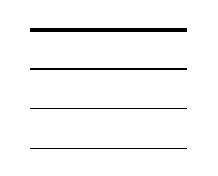
\begin{tikzpicture}
\draw [ultra thick] (0,1) -- (2, 1);
\draw [thick] (0,0.5) -- (2,0.5);
\draw [thin] (0,0) -- (2,0);
\draw [ultra thin] (0, -0.5) -- (2, -0.5);
\end{tikzpicture}
\end{lstlisting}
\end{tabular}

\vspace{1em}
\noindent
Full options include 
ultra thin, very thin, thin, semithick, thick, very
thick, and ultra. Custom widths can also be used.
\par

\noindent

\begin{tikzpicture}
\draw [line width = 12] (0, 0) -- (2,2);
\draw [line width = 0.2 cm] (4, 0.75) -- (5, 0.25);
\end{tikzpicture}
\begin{lstlisting}

\begin{tikzpicture}
\draw [line width = 12] (0, 0) -- (2,2);
\draw [line width = 0.2 cm] (4, 0.75) -- (5, 0.25);
\end{tikzpicture}
\end{lstlisting}

\section{Dashes and dots} % (fold)
\label{sec:dashes_and_dots}
\begin{tabular}{p{3cm}l}

\begin{tikzpicture}[baseline = (current bounding box.east)]
\draw [dashed, ultra thick] (0,1) -- (2,1);
\draw [dashed] (0,0.5) -- (2,0.5);
\draw [dotted] (0,0) -- (2,0);
\end{tikzpicture}
&
\begin{lstlisting}
\begin{tikzpicture}
\draw [dashed, ultra thick] (0,1) -- (2,1);
\draw [dashed] (0,0.5) -- (2,0.5);
\draw [dotted] (0,0) -- (2,0);
\end{tikzpicture}
\end{lstlisting}
\end{tabular}



\section{Colors} % (fold)
\label{sec:colors}
\begin{tabular}{p{3cm}l}

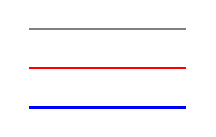
\begin{tikzpicture}[baseline = (current bounding box.east)]
\draw [gray, thick] (0,1) -- (2, 1);
\draw [red, thick] (0,0.5) -- (2, 0.5);
\draw [blue, thick] (0,0) -- (2, 0);
\end{tikzpicture}
&
\begin{lstlisting}
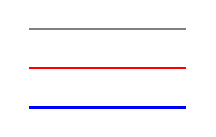
\begin{tikzpicture}
\draw [gray, thick] (0,1) -- (2, 1);
\draw [red, thick] (0,0.5) -- (2, 0.5);
\draw [blue, thick] (0,0) -- (2, 0);
\end{tikzpicture}
\end{lstlisting}
\end{tabular}

\vspace{1em}\noindent
Other colors include red \tikz{\draw [red, line width = 6] (0,0) -- (0.5, 0);}
green \tikz{\draw [green, line width = 6] (0,0) -- (0.5, 0);}
yellow \tikz{\draw [yellow, line width = 6] (0,0) -- (0.5, 0);}
blue \tikz{\draw [blue, line width = 6] (0,0) -- (0.5, 0);}
cyan \tikz{\draw [cyan, line width = 6] (0,0) -- (0.5, 0);}
magenta \tikz{\draw [magenta, line width = 6] (0,0) -- (0.5, 0);}
black \tikz{\draw [black, line width = 6] (0,0) -- (0.5, 0);}
gray \tikz{\draw [gray, line width = 6] (0,0) -- (0.5, 0);}
darkgray \tikz{\draw [darkgray, line width = 6] (0,0) -- (0.5, 0);}
lightgray \tikz{\draw [lightgray, line width = 6] (0,0) -- (0.5, 0);}
brown \tikz{\draw [brown, line width = 6] (0,0) -- (0.5, 0);}
lime \tikz{\draw [lime, line width = 6] (0,0) -- (0.5, 0);}
olive \tikz{\draw [olive, line width = 6] (0,0) -- (0.5, 0);}
orange \tikz{\draw [orange, line width = 6] (0,0) -- (0.5, 0);}
pink \tikz{\draw [pink, line width = 6] (0,0) -- (0.5, 0);}
purple \tikz{\draw [purple, line width = 6] (0,0) -- (0.5, 0);}
teal \tikz{\draw [teal, line width = 6] (0,0) -- (0.5, 0);}
violet \tikz{\draw [violet, line width = 6] (0,0) -- (0.5, 0);}
white \tikz{\draw [white, line width = 6] (0,0) -- (0.5, 0);}
\begin{lstlisting}
\tikz{\draw [<color>, line width = 6] (0,0) -- (0.5, 0);}
\end{lstlisting}

\section{Curves} % (fold)
\label{sec:curves}
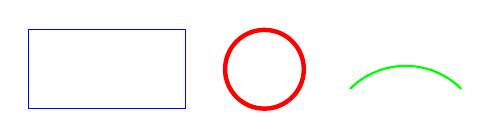
\begin{tikzpicture}
\draw [blue] (0,0) rectangle (2,1);
\draw [red, ultra thick] (3, 0.5) circle [radius = 0.5];
\draw [green, thick] (5.5,0.25) arc [radius = 1, start angle = 45, end angle = 135];
\end{tikzpicture}
\begin{lstlisting}
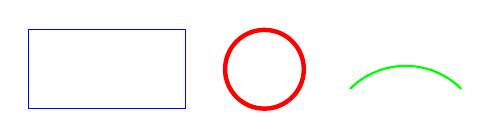
\begin{tikzpicture}
\draw [blue] (0,0) rectangle (2,1);
\draw [red, ultra thick] (3, 0.5) circle [radius = 0.5];
\draw [green, thick] (5.5,0.25) arc [radius = 1, start angle = 45, end angle = 135];
\end{tikzpicture}
\end{lstlisting}
Arc of radius 1 starts at the point (6,0), leaves it at an angle of 45 degrees and stops when its slope is 135 degrees.
To make paths take smoother turns,

\vspace{1em}\noindent
\begin{tabular}{p{3cm}l}

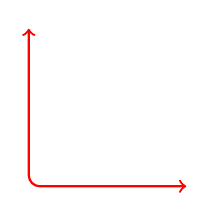
\begin{tikzpicture}[baseline = (current bounding box.east)]
\draw [<->, rounded corners, thick, red] (0,2) -- (0,0) -- (2,0);
\end{tikzpicture}
&
\begin{lstlisting}
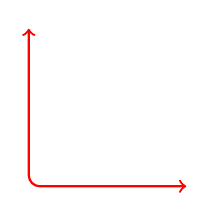
\begin{tikzpicture}
\draw [<->, rounded corners, thick, red] 
	(0,2) -- (0,0) -- (2,0);
\end{tikzpicture}
\end{lstlisting}
\end{tabular}

\vspace{1em}\noindent
Lots of anchor points can be specified explicitly to make a smoother curve.

\vspace{1em}\noindent
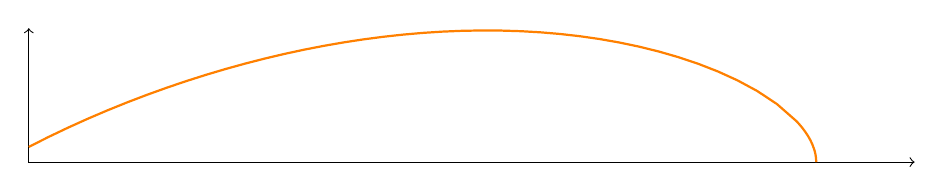
\begin{tikzpicture}[xscale=25,yscale=5]
\draw [<->] (0.6,1.34) -- (0.6,1) -- (1.05,1);
\draw[orange, thick] (0.6, 1.0385) --
(0.61, 1.06372) -- (0.62, 1.08756) -- (0.63, 1.11012) -- 
(0.64,1.13147) -- (0.65, 1.15166) -- (0.66, 1.17074) -- 
(0.67, 1.18874) -- (0.68,1.20568) -- (0.69, 1.22157) -- 
(0.7, 1.23643) -- (0.71, 1.25026) -- (0.72,1.26307) -- 
(0.73, 1.27486) -- (0.74, 1.28561) -- (0.75, 1.29534) -- 
(0.76,1.30402) -- (0.77, 1.31165) -- (0.78, 1.31821) -- 
(0.79, 1.32369) -- (0.8,1.32806) -- (0.81, 1.33131) -- 
(0.82, 1.3334) -- (0.83, 1.33431) -- (0.84,1.334) -- 
(0.85, 1.33244) -- (0.86, 1.32956) -- (0.87, 1.32533) -- 
(0.88,1.31966) -- (0.89, 1.3125) -- (0.9, 1.30373) -- 
(0.91, 1.29325) -- (0.92,1.2809) -- (0.93, 1.26649) -- 
(0.94, 1.24976) -- (0.95, 1.23032) -- (0.96,1.2076) -- 
(0.97, 1.18065) -- (0.98, 1.14763) -- (0.99, 1.1038) -- 
(0.991,1.09836) -- (0.992, 1.09261) -- (0.993, 1.0865) -- 
(0.994, 1.07994) -- (0.995,1.07282) -- (0.996, 1.06497) -- 
(0.997, 1.0561) -- (0.998, 1.04563) -- (0.999,1.03209) -- 
(0.9991, 1.03042) -- (0.9992, 1.02866) -- (0.9993,1.02679) -- 
(0.9994, 1.02478) -- (0.9995, 1.0226) -- (0.9996, 1.02019) -- 
(0.9997,1.01747) -- (0.9998, 1.01424) -- (0.9999, 1.01005) -- 
(0.9999,1.01005) -- (0.99991, 1.00953) -- (0.99992, 1.00898) -- 
(0.99993,1.0084) -- (0.99994, 1.00778) -- (0.99995, 1.0071) -- 
(0.99996,1.00634) -- (0.99997, 1.00549) -- (0.99998, 1.00448) -- 
(0.99999, 1.00317) -- (1,1) ;
\end{tikzpicture}
\begin{lstlisting}
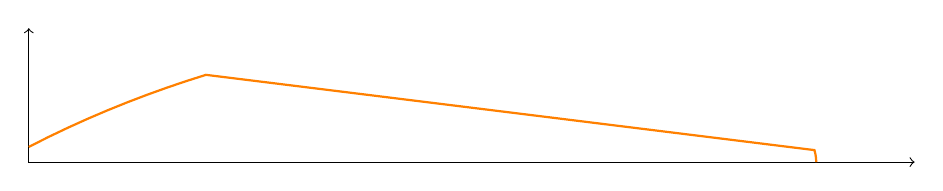
\begin{tikzpicture}[xscale=25,yscale=5]
\draw [<->] (0.6,1.34) -- (0.6,1) -- (1.05,1);
\draw[orange, thick] (0.6, 1.0385) --
(0.61, 1.06372) -- (0.62, 1.08756) -- (0.63, 1.11012) -- 
(0.64,1.13147) -- (0.65, 1.15166) -- (0.66, 1.17074) -- 
(0.67, 1.18874) -- (0.68,1.20568) -- (0.69, 1.22157) -- 
%[... lots of points ...]
(0.9991, 1.03042) -- (0.9992, 1.02866) -- (0.9993,1.02679) -- 
(0.9994, 1.02478) -- (0.9995, 1.0226) -- (0.9996, 1.02019) -- 
(0.9997,1.01747) -- (0.9998, 1.01424) -- (0.9999, 1.01005) -- 
(0.9999,1.01005) -- (0.99991, 1.00953) -- (0.99992, 1.00898) -- 
(0.99993,1.0084) -- (0.99994, 1.00778) -- (0.99995, 1.0071) -- 
(0.99996,1.00634) -- (0.99997, 1.00549) -- (0.99998, 1.00448) -- 
(0.99999, 1.00317) -- (1,1) ;
\end{tikzpicture}
\end{lstlisting}
A simpler way to draw a curve is to specify the inlet and exit points, and the inlet and exit angles. 

\vspace{1em}\noindent
\begin{tabular}{p{3cm}l}

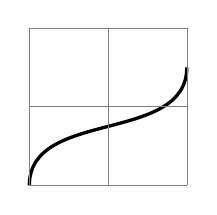
\begin{tikzpicture}[baseline = (current bounding box.east)]
\draw[very thick] (0,0) to [out=90,in=-90] (2,1.5);
\draw[help lines] (0,0) grid (2,2);
\end{tikzpicture}
&
\begin{lstlisting}
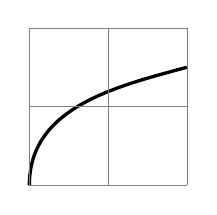
\begin{tikzpicture}
\draw[very thick] (0,0) to [out=90,in=195] (2,1.5);
\draw[help lines] (0,0) grid (2,2);
\end{tikzpicture}
\end{lstlisting}
\end{tabular}

\vspace{1em}\noindent
To decipher the angles, 
\begin{itemize}
	\item Draw a vector at the beginning, (0,0) pointing \emph{right} along the base of the figure. Rotate the vector \emph{counterclockwise} until it is tangent with the drawn curve. The angle turned is the \texttt{\small{out}} angle.
	\item Draw a vector at the end, (2, 1.5) pointing to the \emph{left} parallel to the base of the figure. Rotate the vector \emph{counterclockwise} until it is tangent with the drawn curve. The angle turned is the \texttt{\small{in}} angle. \end{itemize}

\noindent
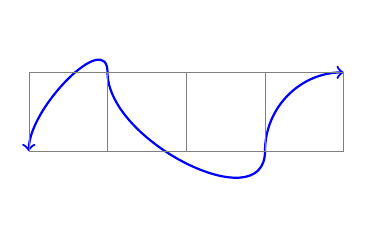
\begin{tikzpicture}
\draw [<->, thick, blue] (0,0) to [out = 90, in = 90] (1,1) [out = -90, in = -90] to (3,0) to [out = 90, in = 180] (4,1);
\draw [help lines] (0,0) grid (4,1);
\end{tikzpicture}
\begin{lstlisting}
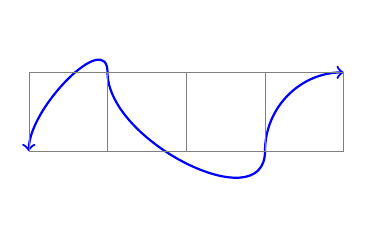
\begin{tikzpicture}
\draw [<->, thick, blue] (0,0) to [out = 90, in = 90] (1,1) [out = -90, in = -90] to (3,0) to [out = 90, in = 180] (4,1);
\draw [help lines] (0,0) grid (4,1);
\end{tikzpicture}
\end{lstlisting}

\section{Plotting functions} % (fold)
\label{sec:plotting_functions}
Ti\emph{k}z has a math engine to plot functions.

\vspace{1em}
\noindent
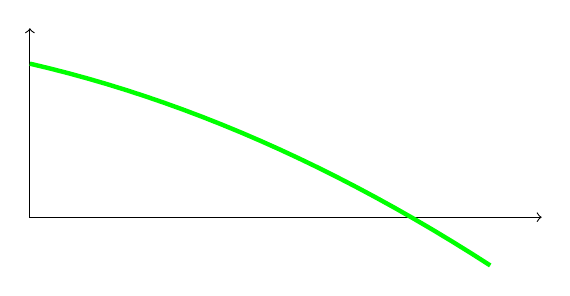
\begin{tikzpicture}[xscale = 13, yscale = 3]
\draw [<->] (0, 0.8) -- (0,0) -- (0.5, 0);
\draw [green, ultra thick, domain = 0:0.45] plot (\x, {0.65 - \x - 2*\x*\x});
\end{tikzpicture}
\begin{lstlisting}
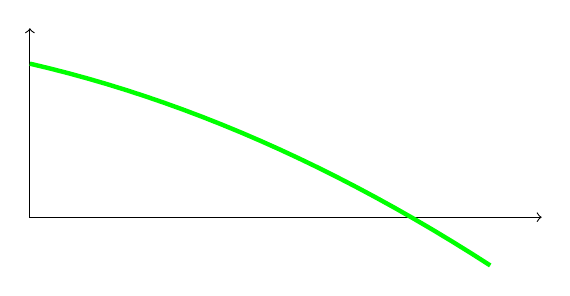
\begin{tikzpicture}[xscale = 13, yscale = 3]
\draw [<->] (0, 0.8) -- (0,0) -- (0.5, 0);
\draw [green, ultra thick, domain = 0:0.45] 
plot (\x, {0.65 - \x - 2*\x*\x});
\end{tikzpicture}
\end{lstlisting}
Available functions include {\small \texttt{factorial(\textbackslash x)}, \texttt{sqrt(\textbackslash x)}, \texttt{pow(\textbackslash x,y)}} ($x^y$){\small, \texttt{exp(\textbackslash x)}, \texttt{ln(\textbackslash x)}, \texttt{log10(\textbackslash x)}, \texttt{log2(\textbackslash x)}, \texttt{abs(\textbackslash x)}, \texttt{mod(\textbackslash x,y)}, \texttt{round(\textbackslash x)}, \texttt{floor(\textbackslash x)}, \texttt{ceil(\textbackslash x)}, \texttt{sin(\textbackslash x)}, (\texttt{sin(\textbackslash x r)}} for radians{\small ), \texttt{cos(\textbackslash x)}, \texttt{cos(\textbackslash x r)}, \texttt{tan(\textbackslash x)}, \texttt{tan(\textbackslash x r)}, \texttt{min(\textbackslash x, y)}, \texttt{max(\textbackslash x, y)}. \par} These functions can be mixed together, along with two provided constants, \texttt{e} =  2.718281828, and \texttt{pi} = 3.141592654.

\vspace{1em}\noindent
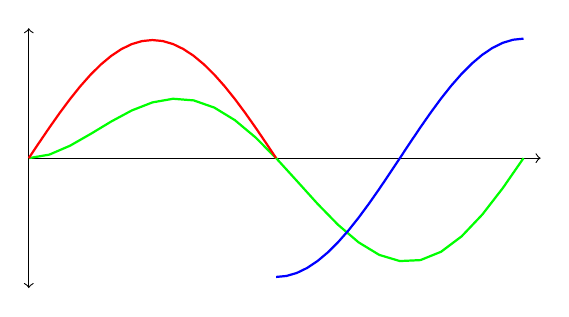
\begin{tikzpicture}[yscale=1.5]
\draw [->] (0,0) -- (6.5,0);
\draw [<->] (0,-1.1) -- (0,1.1);
\draw [green,domain=0:2*pi, thick] plot (\x, {(sin(\x r)* ln(\x+1))/2});
\draw [red,domain=0:pi, thick] plot (\x, {sin(\x r)});
\draw [blue, domain=pi:2*pi, thick] plot (\x, {cos(\x r)*exp(\x/exp(2*pi))});
\end{tikzpicture}
\begin{lstlisting}
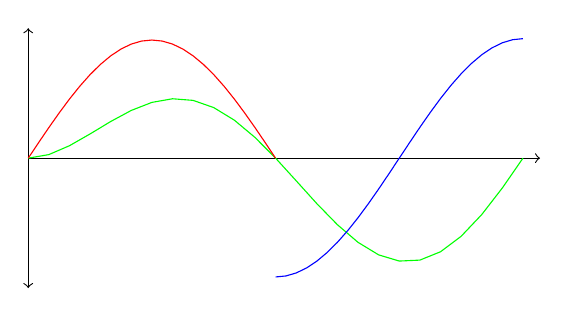
\begin{tikzpicture}[yscale=1.5]
\draw [->] (0,0) -- (6.5,0);
\draw [<->] (0,-1.1) -- (0,1.1);
\draw [green,domain=0:2*pi] plot (\x, {(sin(\x r)* ln(\x+1))/2});
\draw [red,domain=0:pi] plot (\x, {sin(\x r)});
\draw [blue, domain=pi:2*pi] 
plot (\x, {cos(\x r)*exp(\x/exp(2*pi))});
\end{tikzpicture}
\end{lstlisting}

\vspace{1em}\noindent
\begin{tabular}{p{4cm}l}
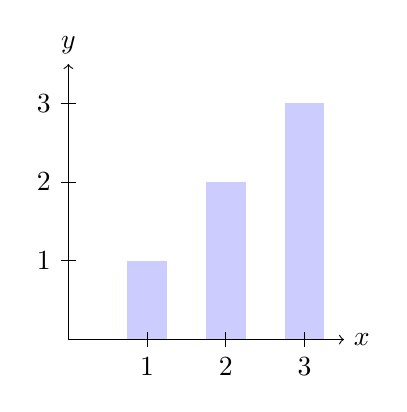
\begin{tikzpicture}[baseline = (current bounding box.east)]
\draw [ycomb, color = blue!20, line width = 0.5 cm]
	plot coordinates{(1,1) (2,2) (3,3)};
\draw (1, -0.1) node [below] {1} -- (1, 0.1)
	(2, -0.1) node [below] {2} -- (2, 0.1)
	(3, -0.1) node [below] {3} -- (3, 0.1);
\foreach \i in {1,2,3}
\draw  (-0.1, \i) node [left] {\i} -- (0.1, \i);
\draw [<->] (0,3.5) node [above] {$y$} 
			-- (0,0) 
			-- (3.5,0) node [right] {$x$} ;
\end{tikzpicture}
&
\begin{lstlisting}
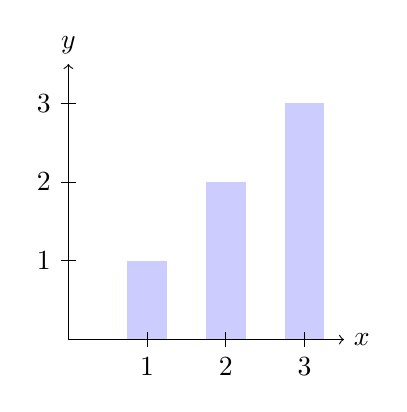
\begin{tikzpicture}
\draw [ycomb, color = blue!20, line width = 0.5 cm]
	plot coordinates{(1,1) (2,2) (3,3)};
\draw (1, -0.1) node [below] {1} -- (1, 0.1)
	(2, -0.1) node [below] {2} -- (2, 0.1)
	(3, -0.1) node [below] {3} -- (3, 0.1);
\foreach \i in {1,2,3}
\draw  (-0.1, \i) node [left] {\i} -- (0.1, \i);
\draw [<->] (0,3.5) node [above] {$y$} 
			-- (0,0) 
			-- (3.5,0) node [right] {$x$} ;
\end{tikzpicture}
\end{lstlisting}
\end{tabular}


\section{Filling areas} % (fold)
\label{sec:filling_areas}
Closed paths can be filled.

\noindent
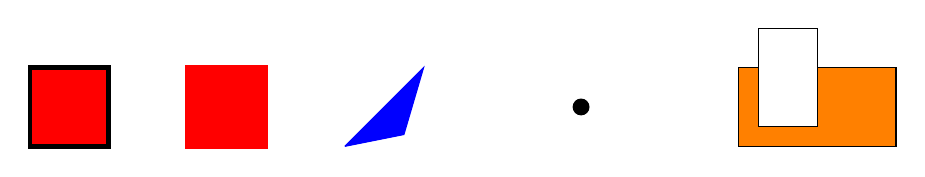
\begin{tikzpicture}
\draw [fill = red, ultra thick] (0,0) rectangle (1,1);
\draw [fill = red, ultra thick, red] (2,0) rectangle (3,1);
\draw [blue, fill = blue] (4,0) -- (5,1) -- (4.75, 0.15) -- (4,0);
\draw [fill] (7, 0.5) circle [radius = 0.1];
\draw [fill = orange] (9,0) rectangle (11,1);
\draw [fill = white] (9.25, 0.25) rectangle (10, 1.5);
\end{tikzpicture}
\begin{lstlisting}
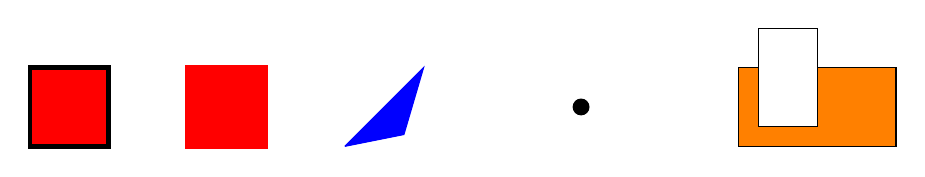
\begin{tikzpicture}
\draw [fill = red, ultra thick] (0,0) rectangle (1,1);
\draw [fill = red, ultra thick, red] (2,0) rectangle (3,1);
\draw [blue, fill = blue] (4,0) -- (5,1) -- (4.75, 0.15) -- (4,0);
\draw [fill] (7, 0.5) circle [radius = 0.1];
\draw [fill = orange] (9,0) rectangle (11,1);
\draw [fill = white] (9.25, 0.25) rectangle (10, 1.5);
\end{tikzpicture}
\end{lstlisting}
To suppress the outline, replace the {\small \texttt{\textbackslash draw}} command with the {\small \texttt{\textbackslash path}} command.

\vspace{1em}
\noindent

\begin{tikzpicture}
\draw [fill = yellow] (0,0) rectangle (1.5,1);
\path [fill = yellow] (2,0) rectangle (3.5,1);
\end{tikzpicture}
\begin{lstlisting}

\begin{tikzpicture}
\draw [fill = yellow] (0,0) rectangle (1.5,1);
\path [fill = yellow] (2,0) rectangle (3.5,1);
\end{tikzpicture}
\end{lstlisting}
Mix \texttt{-}\texttt{-} and \texttt{to} to connect arcs and straight lines.

\noindent

\begin{tikzpicture}
\draw [ultra thick] (0,0) to [out = 87, in = 135] (1,1) -- (0.85, 0.15) -- (0,0);
\draw [ultra thick, fill = purple] (2,0) to [out = 87, in = 135] (3,1) -- (2.85, 0.15) -- (2,0);
\path [fill = purple] (4,0) to [out = 87, in = 135] (5,1) -- (4.85, 0.15) -- (4,0);
\end{tikzpicture}
\begin{lstlisting}

\begin{tikzpicture}
\draw [ultra thick] (0,0) to [out = 87, in = 135] (1,1) -- (0.85, 0.15) -- (0,0);
\draw [ultra thick, fill = purple] (2,0) to [out = 87, in = 135] (3,1) -- (2.85, 0.15) -- (2,0);
\path [fill = purple] (4,0) to [out = 87, in = 135] (5,1) -- (4.85, 0.15) -- (4,0);
\end{tikzpicture}
\end{lstlisting}

\section{Labels in pictures} % (fold)
\label{sec:labels_in_pictures}

\begin{tabular}{p{3cm}l}

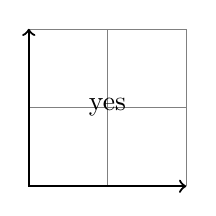
\begin{tikzpicture}[baseline = (current bounding box.east)]
\draw [help lines] (0,0) grid (2,2);
\draw [thick, <->] (0,2) -- (0,0) -- (2,0);
\node at (1,1) {yes};
\end{tikzpicture}
&
\begin{lstlisting}
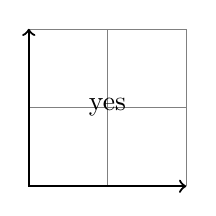
\begin{tikzpicture}
\draw [help lines] (0,0) grid (2,2);
\draw [thick, <->] (0,2) -- (0,0) -- (2,0);
\node at (1,1) {yes};
\end{tikzpicture}
\end{lstlisting}
\end{tabular}

\vspace{1em}\noindent
``yes'' is positioned such that the baseline of the text is centered on {\small \texttt{(1,1)}}. For positioning labels relative to a point,

\vspace{1em}
\noindent
\begin{tabular}{p{3cm}l}

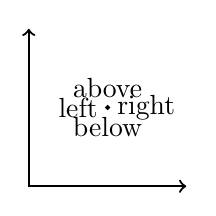
\begin{tikzpicture}[baseline = (current bounding box.east)]
\draw [thick, <->] (0,2) -- (0,0) -- (2,0);
\draw [fill] (1,1) circle [radius = 0.025];
\node [below] at (1,1) {below};
\node [above] at (1,1) {above};
\node [left] at (1,1) {left};
\node [right] at (1,1) {right};
\end{tikzpicture}
&
\begin{lstlisting}
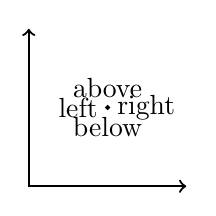
\begin{tikzpicture}
\draw [thick, <->] (0,2) -- (0,0) -- (2,0);
\draw [fill] (1,1) circle [radius = 0.025];
\node [below] at (1,1) {below};
\node [above] at (1,1) {above};
\node [left] at (1,1) {left};
\node [right] at (1,1) {right};
\end{tikzpicture}
\end{lstlisting}

\end{tabular}

\vspace{1em}\noindent
Compound positioning is also possible,

\vspace{1em}
\noindent
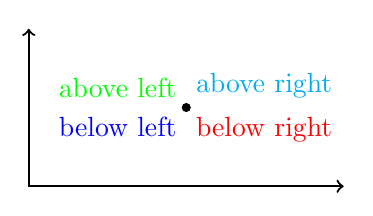
\begin{tikzpicture}[scale = 2]
\draw [thick, <->] (0,1) -- (0,0) --(2,0);
\draw [fill] (1,0.5) circle [radius = 0.025];
\node [below right, red] at (1,0.5) {below right};
\node [above left, green] at (1,0.5) {above left};
\node [below left, blue] at (1,0.5) {below left};
\node [above right, cyan] at (1,0.5) {above right};
\end{tikzpicture}
\begin{lstlisting}
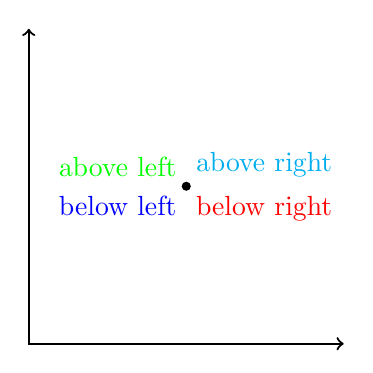
\begin{tikzpicture}[scale = 2.0]
\draw [thick, <->] (0,2) -- (0,0) --(2,0);
\draw [fill] (1,1) circle [radius = 0.025];
\node [below right, red] at (1,1) {below right};
\node [above left, green] at (1,1) {above left};
\node [below left, blue] at (1,1) {below left};
\node [above right, cyan] at (1,1) {above right};
\end{tikzpicture}
\end{lstlisting}

\noindent
Labeling axes and points is also easy.

\vspace{1em}\noindent
\begin{tabular}{p{3cm}l}

\begin{tikzpicture}[scale = 1.5,baseline = (current bounding box.east)]
\draw [thick, <->] (0,1) -- (0,0) --(1,0);
\node [below right] at (1,0) {$x$};
\node [left] at (0,1) {$y$};
\draw [fill] (.4, .6) circle [radius = 0.5 pt];
\node [above right] at (0.4, 0.6) {$A$};
\end{tikzpicture}
&
\begin{lstlisting}
\begin{tikzpicture}[scale = 1.5]
\draw [thick, <->] (0,1) -- (0,0) --(1,0);
\node [below right] at (1,0) {$x$};
\node [left] at (0,1) {$y$};
\draw [fill] (0.4, 0.6) circle [radius = 0.5 pt];
\node [above right] at (0.4, 0.6) {$A$};
\end{tikzpicture}
\end{lstlisting}
\end{tabular}

\vspace{1em}\noindent
Alternatively, nodes can be mixed in the middle of paths.

\vspace{1em}\noindent
\begin{tabular}{p{3cm}l}

\begin{tikzpicture}[scale = 1.5,baseline = (current bounding box.east)]
\draw [thick, <->] (0,1) node [left] {$y$} -- (0,0)
	-- (1,0) node [below right] {$x$};
\draw [fill] (0.4, 0.6) circle [radius = 0.5 pt] 
	node [above right] (0.4, 0.6) {$A$};
\end{tikzpicture}
&
\begin{lstlisting}
\begin{tikzpicture}[scale = 1.5]
\draw [thick, <->] (0,1) node [left] {$y$} -- (0,0)
	-- (1,0) node [below right] {$x$};
\draw [fill] (0.4, 0.6) circle [radius = 0.5 pt] 
	node [above right] (0.4, 0.6) {$A$};
\end{tikzpicture}
\end{lstlisting}
\end{tabular}

\vspace{1em}\noindent
Multiple lines can be added to nodes with \textbackslash\textbackslash, but alignment of the node text must be explicitly specified.

\vspace{1em}\noindent
\begin{tikzpicture}
\draw [thick] (0,0) to (9,0);
\draw (0, -0.2) to (0, 0.2);
\draw (3, -0.2) to (3, 0.2);
\draw (6, -0.2) to (6, 0.2);
\draw (9, -0.2) to (9, 0.2);
\node[align = left, below] at (1.5, -0.5)
	{This is period 1,\\and is aligned\\left.};
\node[align = center, below] at (4.5, -0.5)
	{This is period 2,\\and is aligned\\center.};
\node[align = right, below] at (7.5, -0.5)
	{This is period 3,\\and is aligned\\right.};
\end{tikzpicture}
\begin{lstlisting}
\begin{tikzpicture}
\draw [thick] (0,0) to (9,0);
\draw (0, -0.2) to (0, 0.2);
\draw (3, -0.2) to (3, 0.2);
\draw (6, -0.2) to (6, 0.2);
\draw (9, -0.2) to (9, 0.2);
\node[align = left, below] at (1.5, -0.5)
	{This is period 1,\\and is aligned\\left.};
\node[align = center, below] at (4.5, -0.5)
	{This is period 2,\\and is aligned\\center.};
\node[align = right, below] at (7.5, -0.5)
	{This is period 3,\\and is aligned\\right.};
\end{tikzpicture}
\end{lstlisting}

\section{Naming coordinates} % (fold)
\label{sec:naming_coordinates}
Coordinates can be named with the \texttt{\textbackslash path\dots\textbackslash coordinate} command. Non-contiguous line segments can be drawn by omitting the \texttt{-}\texttt{-} command.

\noindent
\begin{tabular}{p{3cm}l}

\begin{tikzpicture}[baseline = (current bounding box.east)]
\path (0,0) coordinate (origin);
\path (0*72:1 cm) coordinate (P0);
\path (1*72:1 cm) coordinate (P1);
\path (2*72:1 cm) coordinate (P2);
\path (3*72:1 cm) coordinate (P3);
\path (4*72:1 cm) coordinate (P4);

\draw [thick] (P0) -- (P1) -- (P2) -- (P3) -- (P4) -- cycle;
\draw (origin) -- (P0) (origin) -- (P1) (origin) -- 
		(P2) (origin) -- (P3) (origin) -- (P4);
\end{tikzpicture}
&
\begin{lstlisting}
\begin{tikzpicture}
\path (0,0) coordinate (origin);
\path (0*72:1 cm) coordinate (P0);
\path (1*72:1 cm) coordinate (P1);
\path (2*72:1 cm) coordinate (P2);
\path (3*72:1 cm) coordinate (P3);
\path (4*72:1 cm) coordinate (P4);

\draw [thick] (P0) -- (P1) -- (P2) -- (P3) -- (P4) -- cycle;
\draw (origin) -- (P0) (origin) -- (P1) (origin) -- (P2)
	(origin) -- (P3) (origin) -- (P4);
\end{tikzpicture}	
\end{lstlisting}
\end{tabular}

\section{More nodes} % (fold)
\label{sec:more_nodes}
\begin{tabular}{p{3cm}l}
\begin{tikzpicture}[baseline = (current bounding box.east)]
\tikzset{
every node/.style = {circle, thick, draw, text centered,
					fill = blue!20}
}

\path (0:0 cm) node (v0) {$v_0$};
\path (0*72:1 cm) node (v1) {$v_1$};
\path (1*72:1 cm) node (v2) {$v_2$};
\path (2*72:1 cm) node (v3) {$v_3$};
\path (3*72:1 cm) node (v4) {$v_4$};
\path (4*72:1 cm) node (v5) {$v_5$};

\draw (v0) -- (v1) (v0) -- (v2) (v0) -- (v3)
	(v0) -- (v4) (v0) -- (v5);
\end{tikzpicture}
&
\begin{lstlisting}
\begin{tikzpicture}\tikzset{
every node/.style = {circle, thick, draw, text centered,
					fill = blue!20}}

\path (0:0 cm) node (v0) {$v_0$};
\path (0*72:1 cm) node (v1) {$v_1$};
\path (1*72:1 cm) node (v2) {$v_2$};
\path (2*72:1 cm) node (v3) {$v_3$};
\path (3*72:1 cm) node (v4) {$v_4$};
\path (4*72:1 cm) node (v5) {$v_5$};

\draw (v0) -- (v1) (v0) -- (v2) (v0) -- (v3)
	(v0) -- (v4) (v0) -- (v5);
\end{tikzpicture}
\end{lstlisting}
\end{tabular}

\section{Looping} % (fold)
\label{sec:looping}
\begin{tabular}{p{3cm}l}

\begin{tikzpicture}[baseline = (current bounding box.east)]
\foreach \j in {0,...,2}
\foreach \i in {0,...,2}{
	\path (\i,\j) coordinate (x\i\j);
	%\draw (\i, \j) node {$\i,\j$} +(-.5, -.5) rectangle +(.5, .5);
	\fill (x\i\j) circle (1.5pt) node [below] {\i, \j};
}
\end{tikzpicture}
&
\begin{lstlisting}
\begin{tikzpicture}
\foreach \j in {0,...,2}
\foreach \i in {0,...,2}{
	\path (\i,\j) coordinate (x\i\j);
	\fill (x\i\j) circle (1.5pt) node [below] {\i, \j};
}
\end{tikzpicture}
\end{lstlisting}
\end{tabular}

\vspace{1em}\noindent
\begin{tabular}{p{3cm}l}
\begin{tikzpicture}[yscale = 2, baseline = (current bounding box.east)]
\foreach \i / \j in {{1/1}, {2/2}, {3/3}, {4/4}}{
	\path (\i,0) coordinate (X\i);
	\fill (X\i) circle (1pt);
	\path (\j,1) coordinate (Y\j);
	\fill (Y\j) circle (1pt);
}
\foreach \i in {1,...,4}
\foreach \j in {1,...,4}
	\draw (X\i) -- (Y\j);
\end{tikzpicture}
&	
\begin{lstlisting}
\begin{tikzpicture}[yscale=2]
\foreach \i / \j in {{1/1}, {2/2}, {3/3}, {4/4}}{
	\path (\i,0) coordinate (X\i);
	\fill (X\i) circle (1pt);
	\path (\j,1) coordinate (Y\j);
	\fill (Y\j) circle (1pt);
} % Naming coordinates and putting circles
\foreach \i in {1,...,4}
\foreach \j in {1,...,4}
	\draw (X\i) -- (Y\j);
	% Drawing connections
\end{tikzpicture}
\end{lstlisting}
\end{tabular}





% section looping (end)

\section{Examples} % (fold)
\label{sec:examples}

\subsection{Hotelling} % (fold)
\label{sub:hotelling}
\begin{tikzpicture}[xscale = 8]
\draw [red, very thick] (0,0) -- (0.5,0);
\draw [green, very thick] (0.5,0) -- (1,0);
\draw [thick] (0, -0.1) node [below] {0} to (0, 0.1);
\draw [thick] (0.5, -0.1) node [below] {$a=b=$ 1/2} to (0.5, 0.1);
\draw [thick] (1, -0.1) node [below] {1} to (1, 0.1);
\end{tikzpicture}
\begin{lstlisting}
\begin{tikzpicture}[xscale = 8]
\draw [red, very thick] (0,0) -- (0.5,0);
\draw [green, very thick] (0.5,0) -- (1,0);
\draw [thick] (0, -0.1) node [below] {0} to (0, 0.1);
\draw [thick] (0.5, -0.1) node [below] {$a=b=$ 1/2} to (0.5, 0.1);
\draw [thick] (1, -0.1)	node [below] {1} to (1, 0.1);
\end{tikzpicture}
\end{lstlisting}

\subsection{Vertical differentiation} % (fold)
\label{sub:vertical_differentiation}

% subsection vertical_differentiation (end)

\begin{tabular}{p{4cm}l}
\begin{tikzpicture}[yscale=3, baseline = (current bounding box.east)]
\draw[red, very thick] (0,0) to (0, 0.45);
\draw[green, very thick] (0,0.45) to (0, 1);
\draw (-0.1, 0) to (0.1, 0);
\draw[thick] (-0.1, 0.2) to (0.1, 0.2) 
	node [align = left, right] {$q_1$ vendue\\au prix $p_1$};
\draw[thick] (-0.1, 0.8) to (0.1, 0.8) 
	node [align = left, right] {$q_2$ vendue\\au prix $p_2$};
\draw (-0.1, 1) to (0.1, 1);
\node [right] at (0.1, 0.45) {d\'epend de $p_1$ et $p_2$};
\end{tikzpicture} 
& 
\begin{lstlisting}
\begin{tikzpicture}[yscale=3]
\draw[red, very thick] (0,0) to (0, 0.45);
\draw[green, very thick] (0,0.45) to (0, 1);
\draw (-0.1, 0) to (0.1, 0);
\draw[thick] (-0.1, 0.2) to (0.1, 0.2) 
	node [align = left, right] 
	{$q_1$ vendue\\au prix $p_1$};
\draw[thick] (-0.1, 0.8) to (0.1, 0.8) 
	node [align = left, right] 
	{$q_2$ vendue\\au prix $p_2$};
\draw (-0.1, 1) to (0.1, 1);
\node [right] at (0.1, 0.45) {d\'epend de $p_1$ et $p_2$};
\end{tikzpicture} 
\end{lstlisting}
\end{tabular}

\subsection{A curve} % (fold)
\label{sub:a_curve}
\begin{tabular}{p{4cm}l}
\begin{tikzpicture}[scale = 3, baseline = (current bounding box.east)]
\draw [thick, <->] (0,1) node [above] {$V(q)$} -- (0,0) -- (1,0) node [below] {$q$};
\draw [very thick] (0,0) to [out = 90, in = 145] (0.8, 0.9);
\end{tikzpicture}
&
\begin{lstlisting}
\begin{tikzpicture}[scale = 3]
\draw [thick, <->] (0,1) node [above] {$V(q)$} 
	-- (0,0) -- (1,0) node [below] {$q$};
\draw [very thick] (0,0) to 
	[out = 90, in = 145] (0.8, 0.9);
\end{tikzpicture}
\end{lstlisting}
\end{tabular}

\subsection{Tangency} % (fold)
\label{sub:tangency}
\begin{tabular}{p{4cm}l}
\begin{tikzpicture}[scale = 0.75, baseline = (current bounding box.east)]
\draw [help lines] (0,0) grid (5,5);
\draw [black, <->] (0,5) -- (0,0) -- (5,0);
\draw [thick] (0,4) to (4,0);
\draw [dashed, ultra thick] (1, 4) to [out = -90, in = 135] (2,2);
\draw [dashed, ultra thick] (2,2) to [out = -45, in = 180] (4, 1);
\end{tikzpicture}
&
\begin{lstlisting}
\begin{tikzpicture}
\draw [help lines] (0,0) grid (5,5);
\draw [black, <->] (0,5) -- (0,0) -- (5,0);
\draw [thick] (0,4) to (4,0);
\draw [dashed, ultra thick] (1, 4) to 
	[out = -90, in = 135] (2,2);
\draw [dashed, ultra thick] (2,2) to 
	[out = -45, in = 180] (4, 1);
\end{tikzpicture}
\end{lstlisting}
\end{tabular}

\subsection{Consumer surplus} % (fold)
\label{sub:consumer_surplus}

\begin{tikzpicture}
\path [fill = yellow] (0,0)	to (0,5) 
	to [out = -75, in = 150] (3,0.8)
	-- (3,0) -- (0,0); 
\draw [thick, <->] (0,6) node [left] {$P$}
  -- (0,0) node [below left] {$(0,0)$} 
  -- (6,0) node [below] {$Q$};
\draw [thick] (0,5) to [out = -75, in = 150] (3,0.8) 
	to [out = -30, in = 165] (5,0);
\draw [ultra thick, dashed]	(0, 0.8) node [left] {$P^* = .8$} 
	-- (3, 0.8) -- (3,0) node [below] {$Q^* = 3$};
\draw [fill] (3, 0.8) circle [radius = 0.1];
\end{tikzpicture}
\begin{lstlisting}
\begin{tikzpicture}
\path [fill = yellow] (0,0) to (0,5)
	to [out = -75, in = 150] (3,0.8) -- (3,0) -- (0,0); 
\draw [thick, <->] (0,6) node [left] {$P$}
	-- (0,0) node [below left] {$(0,0)$} 
	-- (6,0) node [below] {$Q$};
\draw [thick] (0,5) to [out = -75, in = 150] (3,0.8) 
	to [out = -30, in = 165] (5,0);
\draw [ultra thick, dashed] (0, 0.8) node [left] {$P^* = .8$} 
	-- (3, 0.8) -- (3,0) node [below] {$Q^* = 3$};
\draw [fill] (3, 0.8) circle [radius = 0.1];
\end{tikzpicture}
\end{lstlisting}


\subsection{Lots of curves} % (fold)
\label{sub:lots_of_curves}

\begin{tikzpicture}[domain = 0:0.5, xscale = 13, yscale = 4]
\draw [<->] (0, 1.5) node [left] {\textsc{eur}} -- (0,0) -- (0.6, 0) node [below] {$q$};
\draw [red] plot (\x, {0.25+\x/2 + \x*\x/2}) node [right] {$v_1(x)$};
\draw [blue] plot (\x, {0.025 + \x + \x*\x}) node [right] {$v_2(x)$};
\draw [thin, dashed] plot (\x, {0.275 + 1.5*\x + 1.5*\x *\x});
\draw [thick, domain = 0:0.33666] plot (\x, {0.05+2*\x + 2*\x*\x});
\draw [thick, domain = 0.33666:0.5] plot (\x, 0.5 + \x + \x*\x) node [right] {$2 \text{ min}\left[ v_1, v_2 \right] $};
\end{tikzpicture}
\begin{lstlisting}
\begin{tikzpicture}[domain = 0:0.5, xscale = 13, yscale = 4]
\draw [<->] (0, 2) node [left] {\textsc{eur}} 
	-- (0,0) -- (0.7, 0) node [below] {$q$};
\draw [red] plot (\x, {0.25+\x/2 + \x*\x/2}) node [right] {$v_1(x)$};
\draw [blue] plot (\x, {0.025 + \x + \x*\x}) node [right] {$v_2(x)$};
\draw [thin, dashed] plot (\x, {0.275 + 1.5*\x + 1.5*\x *\x});
\draw [thick, domain = 0:0.33666] plot (\x, {0.05+2*\x + 2*\x*\x});
\draw [thick, domain = 0.33666:0.5] plot (\x, 0.5 + \x + \x*\x) 
	node [right] {$2 \text{ min}\left[ v_1, v_2 \right] $};
\end{tikzpicture}
\end{lstlisting}

\subsection{Simple block diagram} % (fold)
\label{sub:simple_block_diagram}

\begin{tikzpicture}[node distance = 2cm, auto]
\tikzset{
block/.style = {rectangle, thick, draw,
	text width = 3 em, text centered, 
	minimum height = 3 em, fill = blue!20},
line/.style = {draw, ->, thick, >=stealth},
init/.style = {pin edge = {to-, thick, black}}	
}

\node [block, pin = {[init]above:$v_0$}] (a) {$\dfrac{1}{s}$};
\node [left = of a, node distance = 2cm, coordinate] (begin) {};
\node [block, pin = {[init]above:$p_0$}, right = of a] (c)  {$\dfrac{1}{s}$};
\node [right = of c, node distance = 2cm, coordinate] (end) {};
\path [line] (begin) -- node {$a$} (a);
\path [line] (a) -- node {$v$} (c);
\path [line] (c) -- node {$p$} (end);
\end{tikzpicture}
\begin{lstlisting}
\begin{tikzpicture}[node distance = 2cm, auto]\tikzset{
block/.style = {rectangle, thick, draw,
		text width = 3 em, text centered, 
		minimum height = 3 em, fill = blue!20},
line/.style = {draw, ->, thick, >=stealth},
init/.style = {pin edge = {to-, thick, black}}}

\node [block, pin = {[init] above:$v_0$}] 
	(a) {$\dfrac{1}{s}$};
\node [left = of a, node distance = 2cm, coordinate] (begin) {};
\node [block, pin = {[init] above:$p_0$}, right = of a] 
	(c) {$\dfrac{1}{s}$};
\node [right = of c, node distance = 2cm, coordinate] (end) {};

\path [line] (begin) -- node {$a$} (a);
\path [line] (a) -- node {$v$} (c);
\path [line] (c) -- node {$p$} (end);
\end{tikzpicture}
\end{lstlisting}


\subsection{Yin-yang} % (fold)
\label{sub:yin_yang}
\begin{tabular}{p{3cm}l}

\begin{tikzpicture}[scale = 1, baseline = (current bounding box.east)]
\draw (0,0) circle [radius = 1];
\clip (0,0) circle [radius = 1];
\draw [fill] (-1, -1) rectangle (0,1);

\draw [fill] (0, 0.5) circle [radius = 0.5];
\draw [fill, white] (0, -0.5) circle [radius = 0.5];
\draw [fill] (0, -0.5) circle [radius = 0.1];
\draw [fill, white] (0,0.5) circle [radius = 0.1];
\end{tikzpicture}
&
\begin{lstlisting}
\begin{tikzpicture}[scale = 1]
\draw (0,0) circle [radius = 1];
\clip (0,0) circle [radius = 1];
\draw [fill] (-1, -1) rectangle (0,1);

\draw [fill] (0, 0.5) circle [radius = 0.5];
\draw [fill, white] (0, -0.5) circle [radius = 0.5];
\draw [fill] (0, -0.5) circle [radius = 0.1];
\draw [fill, white] (0,0.5) circle [radius = 0.1];
\end{tikzpicture}
\end{lstlisting}
\end{tabular}

\subsection{Set intersection} % (fold)
\label{sub:set_intersection}
\begin{tabular}{p{3cm}l}

\begin{tikzpicture}[scale = 0.75, baseline = (current bounding box.east)]
\draw (-2, 1.5) rectangle (2, -1.5);
\draw (-0.5, 0) circle [radius = 1 cm];
\draw (0.5, 0) circle [radius = 1 cm];
\clip (-0.5, 0) circle [radius = 1 cm];
\clip (0.5, 0) circle [radius = 1 cm];
\draw [fill, blue!20] (-2, 1.5) rectangle (2, -1.5);
\end{tikzpicture}
&
\begin{lstlisting}
\begin{tikzpicture}[scale = 0.75]
\draw (-2, 1.5) rectangle (2, -1.5);
\draw (-0.5, 0) circle [radius = 1 cm];
\draw (0.5, 0) circle [radius = 1 cm];
\clip (-0.5, 0) circle [radius = 1 cm];
\clip (0.5, 0) circle [radius = 1 cm];
\draw [fill, blue!20] (-2, 1.5) rectangle (2, -1.5);
\end{tikzpicture}
\end{lstlisting}
\end{tabular}

\subsection{Even odd rule} % (fold)
\label{sub:even_odd_rule}
\begin{tabular}{p{3cm}l}

\begin{tikzpicture}[even odd rule, rounded corners, 
					x = 1em, y = 1em, scale = 2,
					baseline = (current bounding box.east)]
	\filldraw[fill = blue!50]  		 (0,0) rectangle (1,1)
	[xshift = 0.5em, yshift = 0.5em] (0,0) rectangle (1,1)
	(-1.5,-1.5) rectangle (2,2);
\end{tikzpicture}
&
\begin{lstlisting}
\begin{tikzpicture}[even odd rule, rounded corners, 
			x = 1em, y = 1em, scale = 2]
\filldraw[fill = blue!50] (0,0) rectangle (1,1)
[xshift = 0.5em, yshift = 0.5em] (0,0) rectangle (1,1)
(-1.5,-1.5) rectangle (2,2);
\end{tikzpicture}
\end{lstlisting}
\end{tabular}



\end{document}

